%\documentclass[letterpaper, 10 pt, conference]{ieeeconf}  % Comment this line out
\documentclass[journal, 10pt]{IEEEtran}                                                          % if you need a4paper
%\documentclass[a4paper, 10pt, conference]{ieeeconf}      % Use this line for a4
                                                         % paper
\IEEEoverridecommandlockouts        % This command is only
% needed if you want to
\usepackage{multicol}                              % use the \thanks command
%\overrideIEEEmargins
% See the \addtolength command later in the file to balance the column lengths
% on the last page of the document
% The following packages can be found on http:\\www.ctan.org
\usepackage{graphics} % for pdf, bitmapped graphics files
\usepackage{rotating} % rotate figures
\usepackage{epsfig} % for postscript graphics files
%\usepackage{mathptmx} % assumes new font selection scheme installed
%\usepackage{times} % assumes new font selection scheme installed
\usepackage{amsmath} % assumes amsmath package installed
\usepackage{amssymb} % assumes amsmath package installed
\usepackage{cite}
\usepackage{hyperref}
\usepackage[spanish,mexico]{babel}
\usepackage{float}
\spanishdecimal{.}

\usepackage{atbegshi} % erase first blank page
\AtBeginDocument{\AtBeginShipoutNext{\AtBeginShipoutDiscard}}
%-El titulo debe ser más específico: incluye la metodología que se está aplicando, así como el tipo de datos y la estación de monitoreo correspondiente
\title{Análisis de la calidad del  aire  en  el área metropolitana  de Monterrey (AMM) por medio de conglomerados de variables en estación meteorológica de San Nicolás de los Garza}

\author{Miguel Ángel Chávez Robles \\A01620402}
\begin{document}

\thanks{Miguel Ángel Chávez Robles pertenece al Instituto Tecnológico y de Estudios superiores de Monterrey. Monterrey, N.L. C.P. , 64849, México. 

Este trabajo pertenece a la materia: Aplicación de métodos Multivariados para la Ciencia de Datos. Grupo 1. 

Profesores Dra. Olivia Carrillo Gamboa \& Dr. Daniel Otero Fadul {\tt\small}}


\maketitle

\thispagestyle{empty}
\pagestyle{empty}

\begin{abstract}
La contaminación del aire es un problema que impacta directamente en la calidad de vida de las personas. Sin dudas la contaminación del aire es un serio problema, particularmente en la área metropolitana de Monterrey (AMM). El objetivo del análisis es comprender la interacción que tienen los contaminantes y los indicadores meteorológicos entre si, dando una perspectiva sobre el impacto de la actividad industrial en San Nicolás de los Garza sobre el ambiente y la población del AMM.

\end{abstract}

\begin{IEEEkeywords} 
Conglomerados de variables, contaminantes, análisis multivariado.
\end{IEEEkeywords}

\section{Problematización} \label{problematización}

Nuevo León es uno de los estados mas industriales de México, en este se tiene una alta actividad económica por la variedad de actividades que se desempeñan dentro del mismo. Entre los artículos que se elaboran en el estado se encuentran: vidrio, cemento, acero, cerveza, componentes electrónicos, diversos electrodomésticos, medidores para la industria aeroespacial, entre muchos otros productos \cite{NL} (todo esto sin mencionar la gran actividad agrícola y ganadera del estado, la cual también es bastante alta). Si bien esto es excelente para la economía del estado, su impacto en el ambiente es un problema innegable y creciente; en 2019 el senador Panista Víctor Fuentes solicitó la intervención del gobierno federal en el asunto por medio de una carta enviada a la SEMARNAT, entre sus demandas se encontraba el estudio de las aportaciones de contaminantes de vehículos, transporte público, industrias y construcción, así como implementar acciones para combatir el problema \cite{semarnat}.

No es para menos, pues la contaminación del aire es un problema que impacta directamente en la calidad de vida de las personas, según la Organización Mundial de la Salud es un determinante directo de la salud pública que además tiene impactos socio económicos tales como absentismo laboral y escolar, así como una relación directa con la incidencia de enfermedades respiratorias en la población \cite{efectosSalud}. 

Por si fuera poco, la contaminación del aire también influye directamente en las condiciones climáticas. El cambio climático tiene como principal causa el aumento de la concentración de gases de invernadero \cite{climateChange}. Entre estos se encuentran el \textbf{dióxido de carbono, el metano y el óxido de nitrógeno}. 


\section{Enfoque} \label{enfoque}

Sin dudas la contaminación del aire es un serio problema, particularmente en la área metropolitana de Monterrey (AMM), conformada por este y 12 municipios más, entre ellos San Nicolás de los Garza. Es este último donde se centrará el análisis. San Nicolás de los Garza tiene una actividad industrial, dedicándose principalmente en la producción de cableado, laminados y acero , logrando una actividad económica de 2.89 mil millones de dólares en exportaciones en 2020\cite{dataméxico} por lo que es de particular interés saber como afectan los contaminantes a esta región, y sobre todo como estos interactúan entre si con así como con los indicadores meteorológicos para poder así comprender los efectos que la actividad industrial tiene sobre los mismos y en consecuencia sobre la población del AMM.  

En concreto son de interés las medidas correspondientes a:
\begin{itemize}
    \item Monóxido de carbono (CO)
    \item Dióxido de carbono (CO$_2$)
    \item Dióxido de nitrógeno (NO$_2$)
    \item Óxido de nitrógeno (NO$_x$)
    \item Ozono (O$_3$) (lectura a nivel del suelo)
    \item Material particulado PM$_{10}$ (material particulado como cenizas o polvo con un diámetro menor a 10 $\mu$m
    \item Material particulado PM$_{2.5}$ (material particulado como cenizas o polvo con un diámetro menor a 2.5 $\mu$m
    \item Dióxido de azufre (SO$_2$)
    \item Plomo (Pb)
    \item Hidrocarburos contaminantes tales como:
    \subitem Metano (CH$_4$)
    \subitem Benceno (C$_6$H$_6$)
\end{itemize}
pues estos son los contaminantes que han sido reconocidos como causantes de contaminación ambiental. 



El análisis se centra en un periodo de tiempo obtenido de una base de datos proporcionada por el Sistema Integral de Monitoreo Ambiental (por sus siglas SIMA) perteneciente al Gobierno del Estado de Nuevo León. Esta base de datos cuenta con lecturas hechas cada hora sobre el nivel de contaminantes, así como de indicadores meteorológicos de una estación ubicada en San Nicolás de los Garza, así como una estampa de tiempo para cada registro. Los datos disponibles corresponden a lecturas que se realizaron cada hora desde 2017 el primero de enero de 2017 hasta el 31 de diciembre de 2020.  




\section{Propósito} \label{proposito}

Como se mencionó en la sección \ref{enfoque}, el objetivo del análisis es comprender la interacción que tienen los contaminantes y los indicadores meteorológicos entre si, dando una perspectiva sobre el impacto de la actividad industrial en San Nicolás de los Garza sobre el ambiente y la población del AMM. La técnica a utilizar se conoce como conglomerados de variables, se trata de un método jerárquico que calcula la similitud que existe entre las variables, agrupando las que guardan correlación entre si \cite{appliedMulti}.   

A diferencia de otras técnicas existentes, el análisis de conglomerados no parte de suposiciones previas sobre los datos (tales como el número de grupos a considerar). Se busca un agrupamiento natural de los datos a partir de las medidas de similitud encontradas, por lo que es una técnica bastante adecuada para realizar análisis exploratorio \cite{appliedMulti}. 

Para realizar un análisis de conglomerados es necesario conocer las medidas de similitud o distancias entre las variables. En el caso de conglomerados de variables, se requieren coeficientes de asociación como lo es la correlación, para posteriormente obtener la distancia entre las variables a partir de este mismo , cabe mencionar que esta última puede variar dependiendo de si se calcula usando la correlación o la correlación absoluta \cite{minitab_n.d.}.

Este análisis responde las preguntas: \begin{itemize}
    \item ¿Que variables están asociadas entre si?
    \item ¿Cual es la medida de similitud entre las mismas?
    \item  ¿Existe relación entre la variable $x_i$ y la $x_j$? 
    \item ¿Que agrupación de variables aporta más información en la menor cantidad de grupos posible?
\end{itemize}


\section{Información}\label{informacion}
\subsection{Vista general de el análisis de grupos de variables}\label{overview}
La técnica en cuestión es útil para responder a los cuestionamientos planteados en la sección \ref{proposito}, pues como se menciona en la sección \ref{enfoque} la cantidad de datos a analizar es bastante grande, y estos se desglosan en un total de 15 variables continuas y 1 categórica (la estampa de tiempo), por lo que buscar representar información con alta similitud en un menor número de variables sería algo natural, y por medio de los grupos de variables se comprende la relación que estas tienen favoreciendo este propósito. 

\subsection{Métodos de enlace}

Son adecuados para agrupar tanto variables como observaciones. En el caso de los métodos jerárquicos, inicialmente se tienen tantos grupos como observaciones (en este caso variables), y conforme avanza el proceso se agrupan entre si por similitud, terminando con un solo gran grupo en el último paso. Esto no es muy útil; tener tantos grupos como variables no aporta información, pues solo se están observando por separado, por el contrario tener un solo grupo ignora la distancia que existe entre los mismos y por ende es como observar a todas las variables como si solo fuese una. Es aquí donde entra el concepto de un dendograma, esta figura ilustra todos los posibles agrupamientos que se pueden hacer dadas $n$ variables. Esto lo hace mostrando la distancia entre los grupos en el eje $y$ y el objeto en cuestión en el eje $x$. Un ejemplo de este tipo de figura se puede observar en la figura \ref{fig:dendoGen}. Un buen criterio para escoger un número adecuado de grupos es leer el dendograma, observar donde sucede el cambio más pronunciado en distancia, y tomar el número de grupos previo a este cambio (pues es allí donde crece más la similitud entre los grupos). A continuación se explican los métodos de enlace entre los grupos en base a los que se calcula la distancia usados en el análisis. 

\subsubsection{De enlace simple}\label{simple}
También se conoce como de vecino más cercano. Los grupos se forman uniendo las entidades mas cercanas con su vecino más cercano donde el vecino más cercano es el que tiene la menor distancia. Este método de enlace define la distancia entre un grupo $U$ y un grupo $V$ de cualquier otro grupo $W$ como:

\begin{equation}\label{eq:simple}
d_{(U V)W} = min\{5d_{UW}, d_{VW}\}
\end{equation}
\cite{appliedMulti}

\subsubsection{De enlace completo}\label{complete}
Funciona de una manera muy similar a el enlace simple, pero a diferencia de este entre cada paso se computa la distancia entre los elementos más distantes de un grupo, es decir toman el vecino más lejano. Entonces, la ecuación \ref{eq:simple} se convierte en:
\begin{equation}\label{eq:comlete}
d_{(U V)W} = max\{5d_{UW}, d_{VW}\}
\end{equation}
\cite{appliedMulti}


\subsubsection{De enlace promedio}\label{avg}
Este método de enlace trata la distancia entre grupos como la distancia promedio entre pares de elementos de los grupos en cuestión. Toma el elemento más cercano y lo agrega a su grupo. Su fórmula de distancia está dada por:
\begin{equation}\label{eq:avg}
    d_{(U V)W}=\frac{\sum_{i}\sum_{k}d_{ik}}{N_{(UV)}N_W}
\end{equation}
Dónde $N_{(UV)}$ y $N_W$ son el número de elementos en el grupo $N_{(UV)}$ y $N_W$ respectivamente\cite{appliedMulti}.

\subsection{Enlace Ward}\label{ward}
Este método de enlace se basa en minimizar la pérdida de información al unir 2 grupos. Dicho de otra forma, busca que los grupos representen la mayor cantidad de información haciendo la menor cantidad de uniones posible. Se basa en la suma de errores cuadráticos. En cada paso, se crea el grupo que crea la suma de errores cuadráticos más chica\cite{appliedMulti}. 

\subsection{Periodo temporal usado}

Como se menciona en la sección \ref{enfoque} los datos cubren desde el primero de enero de 2017 hasta el 31 de diciembre de 2020, siendo un total de 35064 registros. Sin embargo, existen periodos con una pérdida de información considerable, tanto dentro de las observaciones como de las propias variables, de hecho no existe una sola variable (a excepción de fecha) que cuente con todos sus registros. Existen meses enteros con lecturas de ciertas variables faltantes. En concreto las variables NO${_2}$ y NO${_x}$ cuentan con un número tan pequeño de observaciones que han sido excluidas del análisis. Las estadísticas descriptivas del periodo 2017-2019 se pueden observar en la figura \ref{fig:descriptiva}. 

Debido a que este análisis se beneficia de tener la mayor cantidad de información posible, no es viable tomar la base de datos entera ya que se requieren registros donde estén presentes todas las variables a analizar, por lo que se delimita un subconjunto para trabajar. Tras realizar un análisis exploratorio se determina que el periodo Agosto 2018 a Julio 2019 es adecuado. Tomar este subconjunto permite tener datos más consistentes. Cabe aclarar que la variable NEWD (North East Wind Direction) se elimina casi por completo, quedando solo con 10 registros. Pese a esto, sigue siendo el periodo más estable encontrado para realizar el análisis. Las estadísticas descriptivas del periodo 01/08/2018-31/07/2019 se pueden observar en la figura \ref{fig:descriptiva2}. 

\section{Razonamiento} \label{razonamiento}

Tras definir el conjunto de datos para el análisis, se realiza el mismo con cada uno de los métodos de enlace descritos en las secciones \ref{simple}, \ref{complete}, \ref{avg} y \ref{ward}. Se aplicó la siguiente metodología en cada uno de los métodos: 

\begin{enumerate}
    \item Obtener el dendograma completo para el método, así como la matriz de semejanzas y distancias
    \item Observar en que paso sucede el salto de distancia más grande
    \item Tomar el número de grupos previo a este salto
    \item Generar el dendograma con el nuevo número de grupos
\end{enumerate}

Los resultados obtenidos usando esta metodología se pueden observar en las figuras \ref{fig:matrizSimple}, \ref{fig:gramaSimple}, \ref{fig:matrizSimpleFinal} y  \ref{fig:dendogramaSimple} para el método de enlace simple, \ref{fig:matrizCompleto}, \ref{fig:gramaCompleto}, \ref{fig:matrizCompletoFinal} y  \ref{fig:dendogramaCompleto} para el método de enlace completo, \ref{fig:matrizAvg}, \ref{fig:gramaAvg}, \ref{fig:matrizAvgFinal} y  \ref{fig:dendogramaAvg} para el método de enlace por promedio y \ref{fig:matrizWard}, \ref{fig:gramaWard}, \ref{fig:matrizWardFinal} y  \ref{fig:dendogramaWard} para el método de enlace Ward. 

\section{Conclusiones y Recomendaciones} \label{conclusiones}

En la sección \ref{overview} se detalla que se espera obtener de estos agrupamientos, por lo que el método que se pueda considerar más significativo es el que haya obtenido una combinación de: diferencia menor de distancia entre los grupos, mayor similitud y menor número de conglomerados tras haber fijado el número de grupos. En este caso los análisis más significativos son tanto el de enlace simple como el de enlace completo, esto es esperable pues la manera en la que funcionan es bastante similar. Si bien es cierto que los resultados muestran que el nivel de semejanza es ligeramente mayor en el caso del método de enlace simple, la mejora es tan baja que es despreciable, ambos análisis son igualmente significativos, aunque personalmente prefiero el método de enlace simple. Ambos métodos agruparon las variables de la misma manera; los conglomerados finales llevan a concluir que:
\begin{enumerate}
    \item PM$_{10}$ y PM$_{2.5}$ presentan similitud. Ambas hacen referencia a material particulado, aunque es interesante que ambos se presenten en cantidades correlacionadas pues dependiendo de la actividad en la región este podría no ser el caso 
    \item O$_3$, Radiación solar, NO y la temperatura presentan similitudes. Si bien esto es de esperarse de la radiación solar y la temperatura, el hecho de que gases contaminantes también lo estén sugiere que los niveles de actividad industrial afectan a el AMM
    \item La velocidad del viento, el monóxido de carbono y la lluvia no presentan similitud con ninguna otra variable
    \item La humedad relativa y la presión atmosférica presentan similitudes, esto tiene sentido pues la humedad relativa aumenta conforme el aire se enfría, mientras que la presión atmosférica hace referencia a la fuerza que ejerce el aire
\end{enumerate}

Haciendo énfasis en el segundo hallazgo, se sugiere investigar si la similitud encontrada entre esas variables es un fenómeno de causa efecto, y si es así que se tomen las medidas pertinentes, pues tener niveles altos de radiación solar y temperatura en consecuencia de la actividad industrial del AMM perjudicaría a la población. 

\bibliographystyle{apalike}
\bibliography{bibliografia.bib}

\section{Apéndice}
\begin{figure}[H]
    \centering
    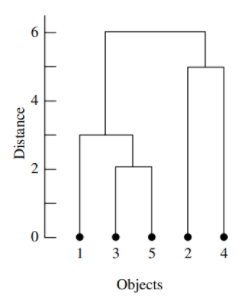
\includegraphics[scale=0.5]{dendograma.png}
    \caption{Ejemplo de dendograma}
    \label{fig:dendoGen}
\end{figure}


\begin{figure}[H]
    \centering
    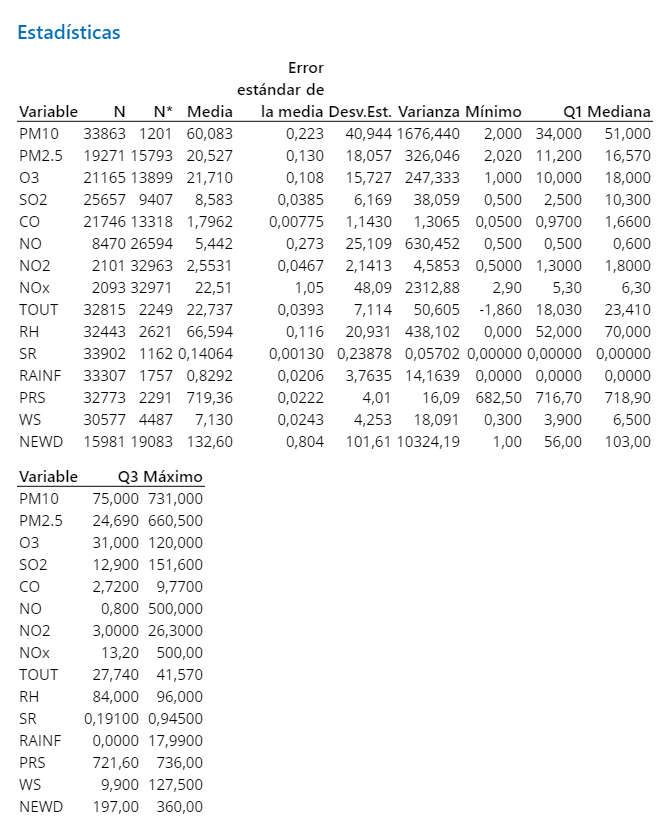
\includegraphics[scale=.3]{descriptivaTotal.png}
    \caption{Estadísticas descriptivas de la base de datos entera}
    \label{fig:descriptiva}
\end{figure}

\begin{figure}[H]
    \centering
    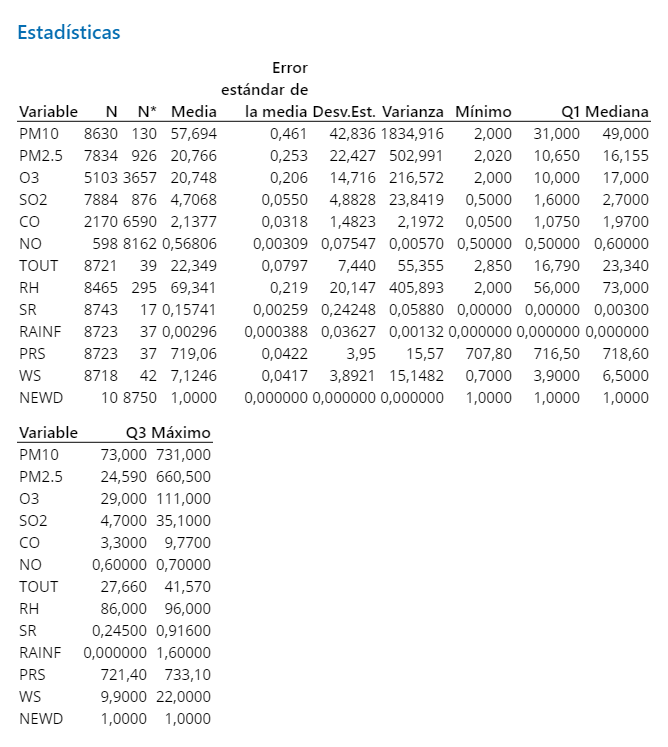
\includegraphics[scale=.3]{descriptiva.png}
    \caption{Estadísticas descriptivas del subconjunto seleccionado}
    \label{fig:descriptiva2}
\end{figure}



\begin{figure}[H]
    \centering
    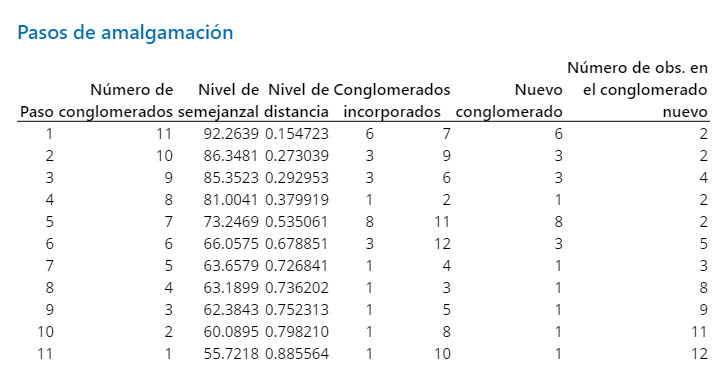
\includegraphics[scale=.3]{matrizSimple.png}
    \caption{Matriz con enlace simple}
    \label{fig:matrizSimple}
\end{figure}

\begin{figure}[H]
    \centering
    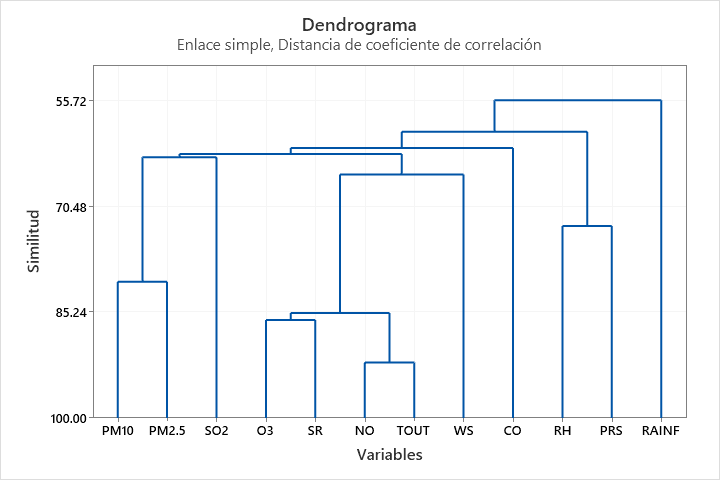
\includegraphics[scale=.3]{gramaSimple.png}
    \caption{Dendograma preliminar usando enlace simple}
    \label{fig:gramaSimple}
\end{figure}

\begin{figure}[H]
    \centering
    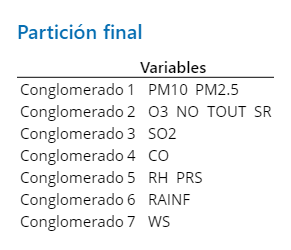
\includegraphics[scale=.3]{matrizSimpleFinal.png}
    \caption{Matriz de grupos final con enlace simple}
    \label{fig:matrizSimpleFinal}
\end{figure}

\begin{figure}[H]
    \centering
    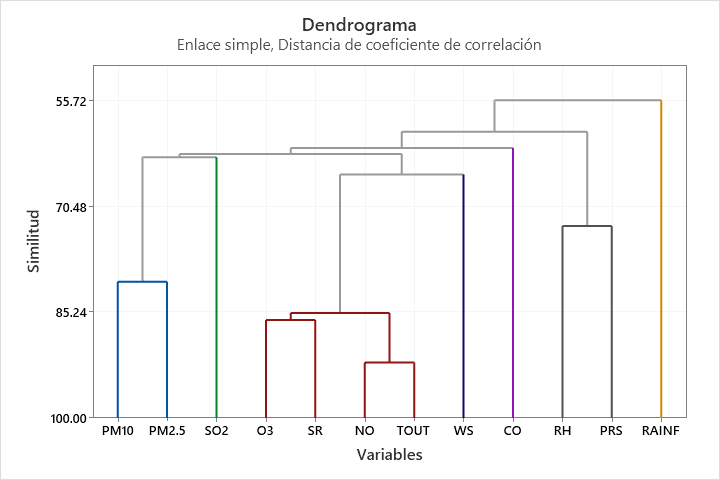
\includegraphics[scale=.3]{dendogramaSimple.png}
    \caption{Dendograma usando enlace simple}
    \label{fig:dendogramaSimple}
\end{figure}



\begin{figure}[H]
    \centering
    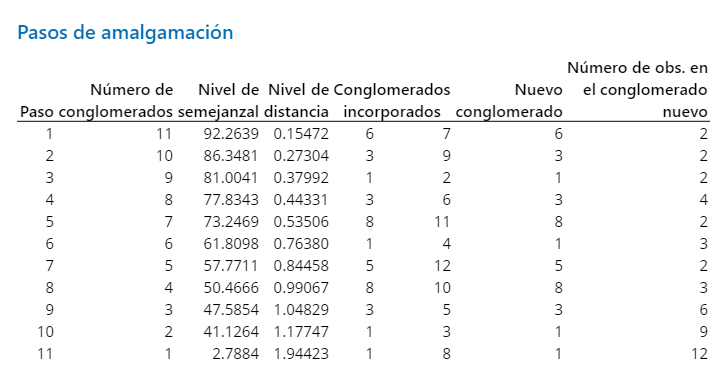
\includegraphics[scale=.3]{matrizCompleto.png}
    \caption{Matriz con enlace completo}
    \label{fig:matrizCompleto}
\end{figure}

\begin{figure}[H]
    \centering
    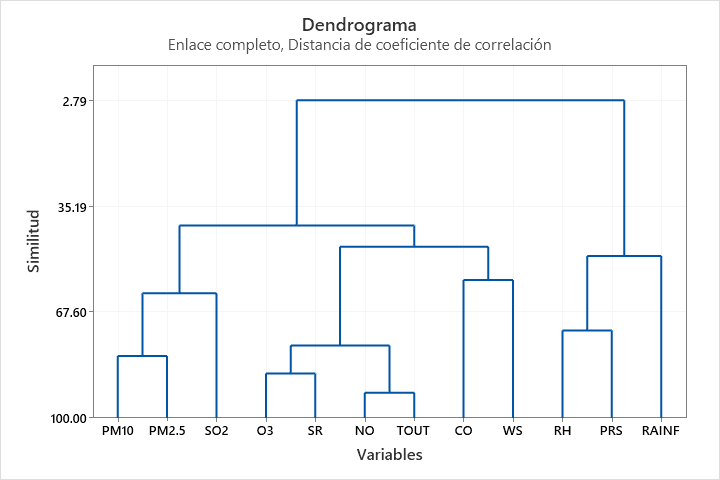
\includegraphics[scale=.3]{gramaCompleto.png}
    \caption{Dendograma preliminar usando enlace completo}
    \label{fig:gramaCompleto}
\end{figure}

\begin{figure}[H]
    \centering
    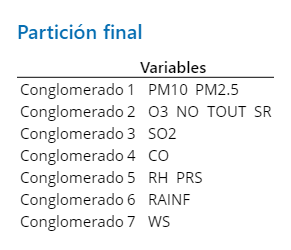
\includegraphics[scale=.3]{matrizCompletoFinal.png}
    \caption{Matriz de grupos final con enlace completo}
    \label{fig:matrizCompletoFinal}
\end{figure}

\begin{figure}[H]
    \centering
    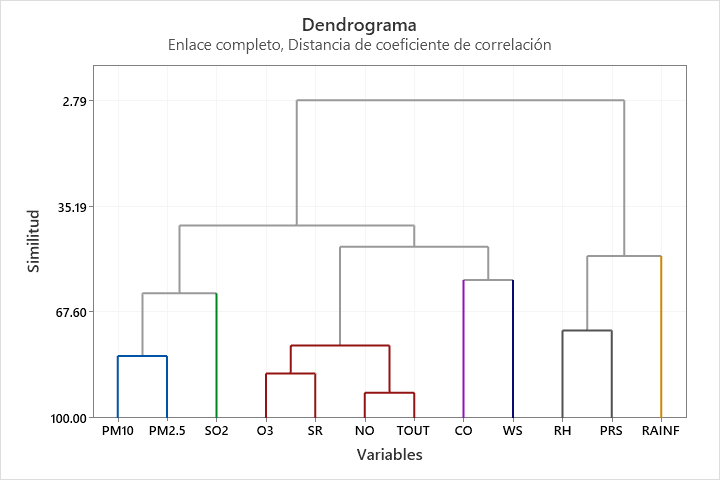
\includegraphics[scale=.3]{dendogramaCompleto.png}
    \caption{Dendograma usando enlace completo}
    \label{fig:dendogramaCompleto}
\end{figure}








\begin{figure}[H]
    \centering
    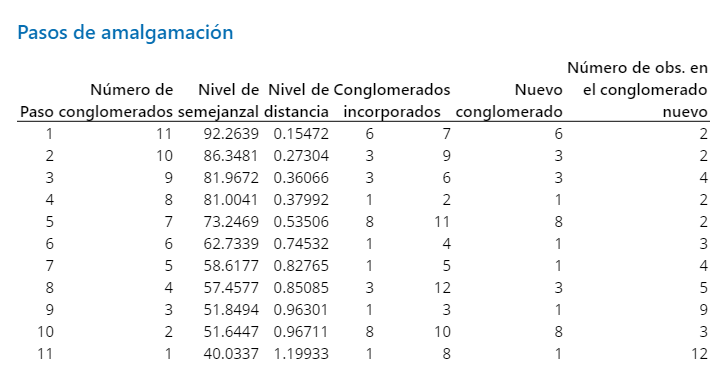
\includegraphics[scale=.3]{matrizAvg.png}
    \caption{Matriz con enlace de promedios}
    \label{fig:matrizAvg}
\end{figure}

\begin{figure}[H]
    \centering
    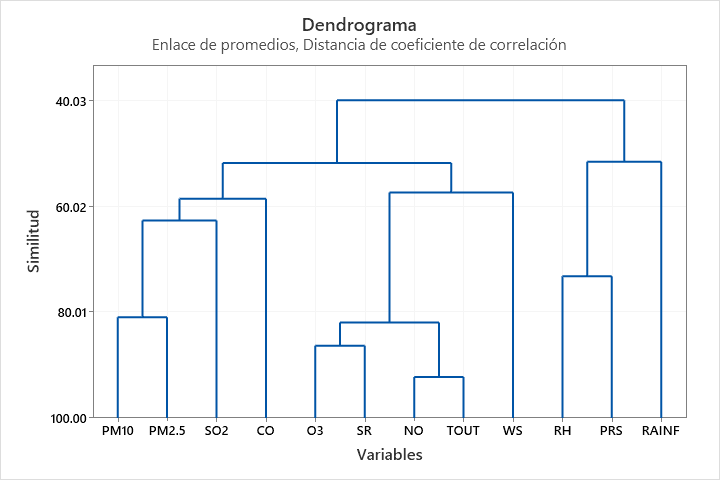
\includegraphics[scale=.3]{gramaPromedio.png}
    \caption{Dendograma preliminar usando enlace de promedios}
    \label{fig:gramaAvg}
\end{figure}

\begin{figure}[H]
    \centering
    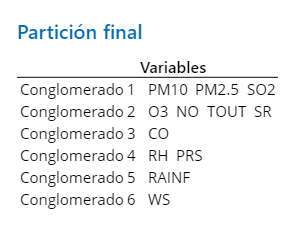
\includegraphics[scale=.3]{matrizAvgFinal.png}
    \caption{Matriz de grupos final con enlace de promedios}
    \label{fig:matrizAvgFinal}
\end{figure}

\begin{figure}[H]
    \centering
    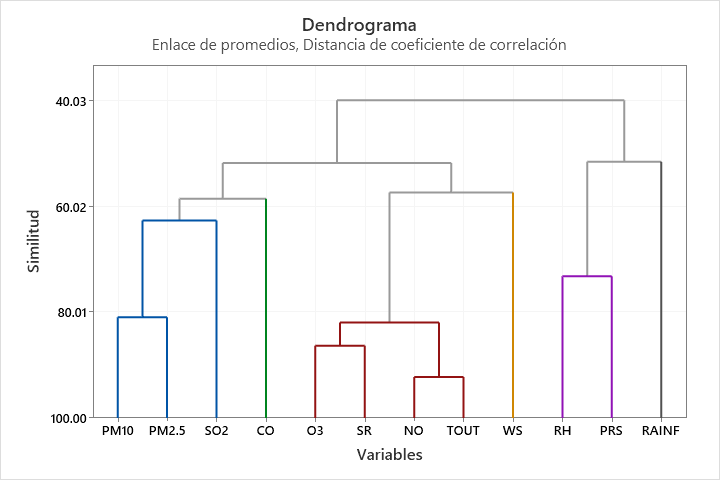
\includegraphics[scale=.3]{dendogramaAvg.png}
    \caption{Dendograma usando enlace de promedios}
    \label{fig:dendogramaAvg}
\end{figure}



\begin{figure}[H]
    \centering
    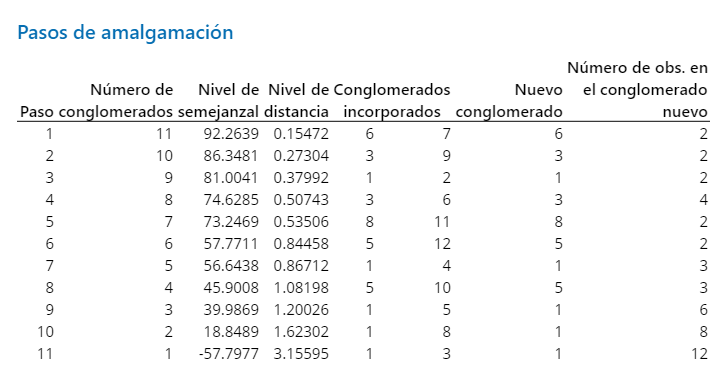
\includegraphics[scale=.3]{matrizWard.png}
    \caption{Matriz con enlace Ward}
    \label{fig:matrizWard}
\end{figure}

\begin{figure}[H]
    \centering
    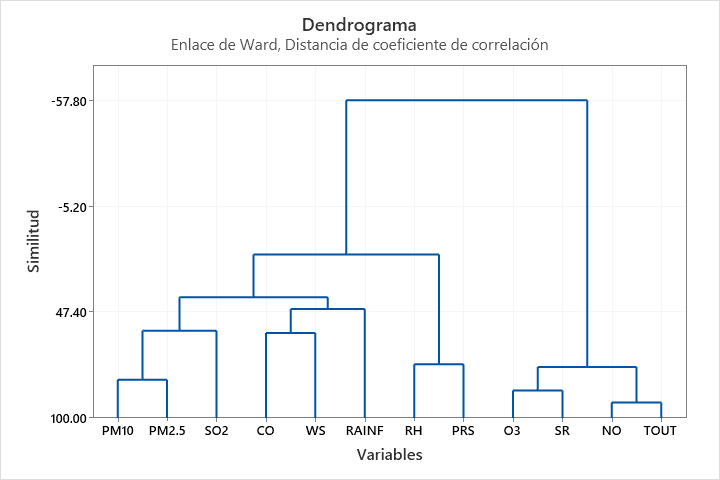
\includegraphics[scale=.3]{gramaWard.png}
    \caption{Dendograma preliminar usando enlace Ward}
    \label{fig:gramaWard}
\end{figure}

\begin{figure}[H]
    \centering
    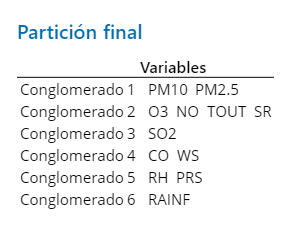
\includegraphics[scale=.3]{matrizWardFinal.png}
    \caption{Matriz de grupos final con enlace Ward}
    \label{fig:matrizWardFinal}
\end{figure}

\begin{figure}[H]
    \centering
    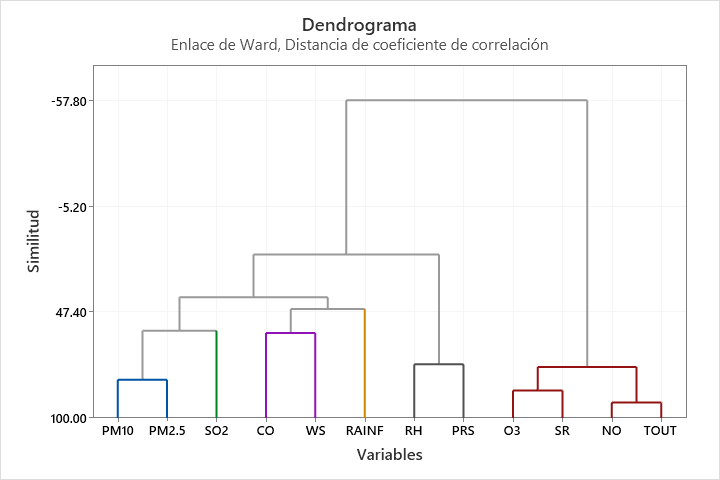
\includegraphics[scale=.3]{dendogramaWard.png}
    \caption{Dendograma usando enlace Ward}
    \label{fig:dendogramaWard}
\end{figure}

\end{document}